\section{Interface graficzny}
    Aplikacjach graficzna na komputery osobiste została napisana w języku \textit{C++} z wykorzystaniem biblioteki \textit{Qt}.
    Poniżej (rys. \ref{fig:gui}) przedstawiono poglądowe zdjęcie aplikacji:

    \begin{figure}[!ht]
        \centering
        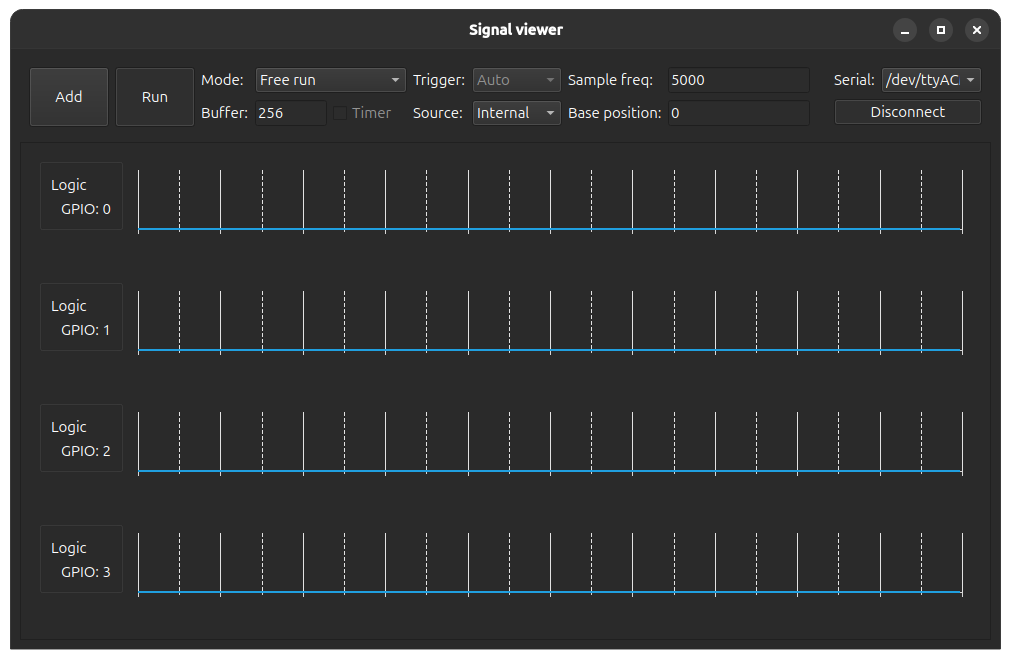
\includegraphics[width = 0.8\textwidth]{GUI.png}
        \caption{Zdjęcie aplikacji graficznej}
        \label{fig:gui}
    \end{figure}

    Dzięki wykorzystaniu biblioteki \textit{Qt}, aplikacja dynamicznie dostosowuje się do motywów systemowych co zaprezentowano na rysunku \ref{fig:gui_white}.
    \begin{figure}[!ht]
        \centering
        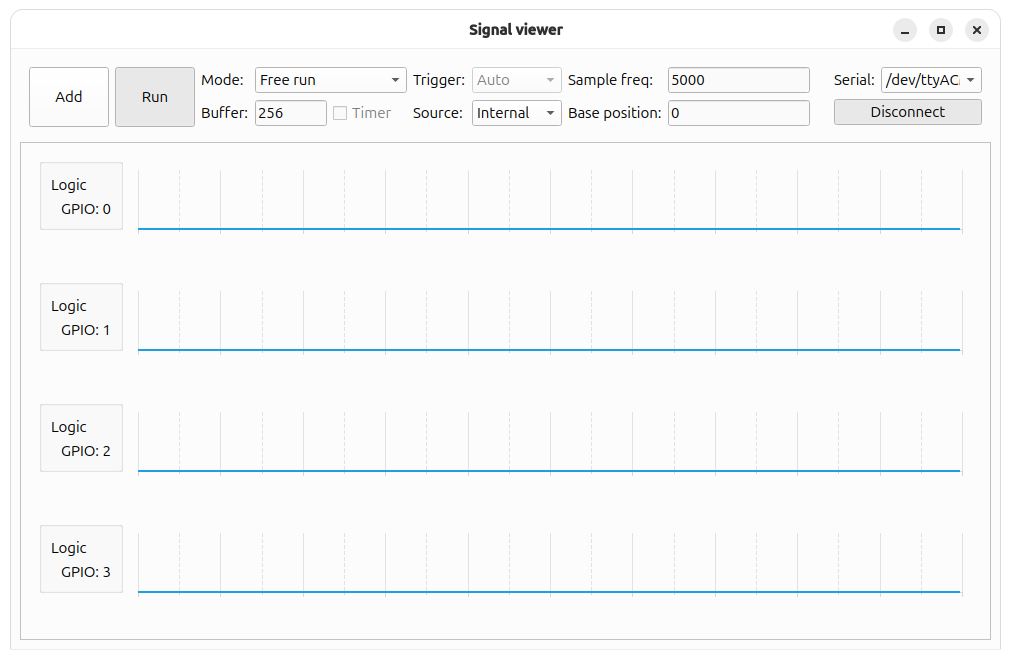
\includegraphics[width = 0.8\textwidth]{GUI_white.png}
        \caption{Zdjęcie aplikacji graficznej}
        \label{fig:gui_white}
    \end{figure}


    \subsection{Ustawienia analizatora}
        Z pomocą interfejsu użytkownika może, zmieniać ustawienia analizatora stanów logicznych takie jak:
        \begin{enumerate}
            \item tryb pracy analizatora:
            \begin{itemize}
                \item ,,Free run'' -- tryb pierścieniowy, po zapełnieniu całego bufora stare dane zostają nadpisane przez nowe
                \item ,,Counted''  -- w tym trybie układ zbiera dokładnie określoną liczbę próbek zapisaną w polu \textit{Buffer}
            \end{itemize}
            \item źródło wyzwalania:
            \begin{itemize}
                \item Trigger   -- dwa dodatkowe piny służące wyłącznie do wyzwalania
                \item GPIO      -- wyprowadzenia pomiarowe od 0 do 15
                \item Internal  -- wyzwalanie wewnętrznym zegarem Raspberry PI PICO
            \end{itemize}
            \item częstotliwość próbkowania:
            \begin{itemize}
                \item w przypadku wyzwalania wewnętrznym zegarem to ustawienie odpowiada za częstotliwość wyzwalania
                \item jeśli znacznik \textit{Timer} jest oznaczony, pole \textit{Sample freq} odpowiada za częstotliwość pomiaru czasu
            \end{itemize}
        \end{enumerate}

    \subsection{Wyświetlanie wykresów}
        W aplikacji można dynamicznie modyfikować liczbę wykresów.
        Po kliknięciu w przycisk ,,Add'' otwiera się dodatkowe okienko (rys. \ref{fig:gui_addPlot}) z poziomu,
        którego użytkownik może dodawać różnego rodzaju wykresy.
        \begin{figure}[!ht]
            \centering
            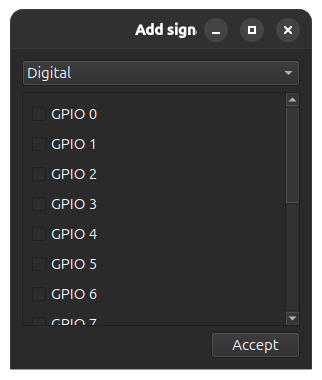
\includegraphics[width = 0.4\textwidth]{GUI_addPlot.png}
            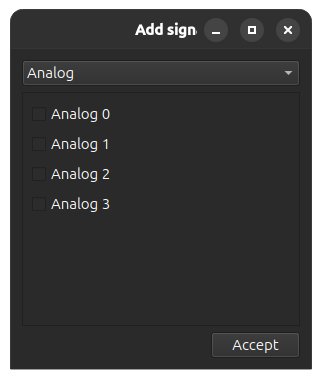
\includegraphics[width = 0.4\textwidth]{GUI_addAnalog.png}
            \caption{Okienko dodawania wykresów}
            \label{fig:gui_addPlot}
        \end{figure}

        Wykresy można także dynamicznie usuwać, po kliknięciu w niechciany prawym przyciskiem myszy pojawia się rozwijane menu z opcją \textit{Remove}.
        Co zaprezentowano na rysunku poniżej.

        \begin{figure}[!ht]
            \centering
            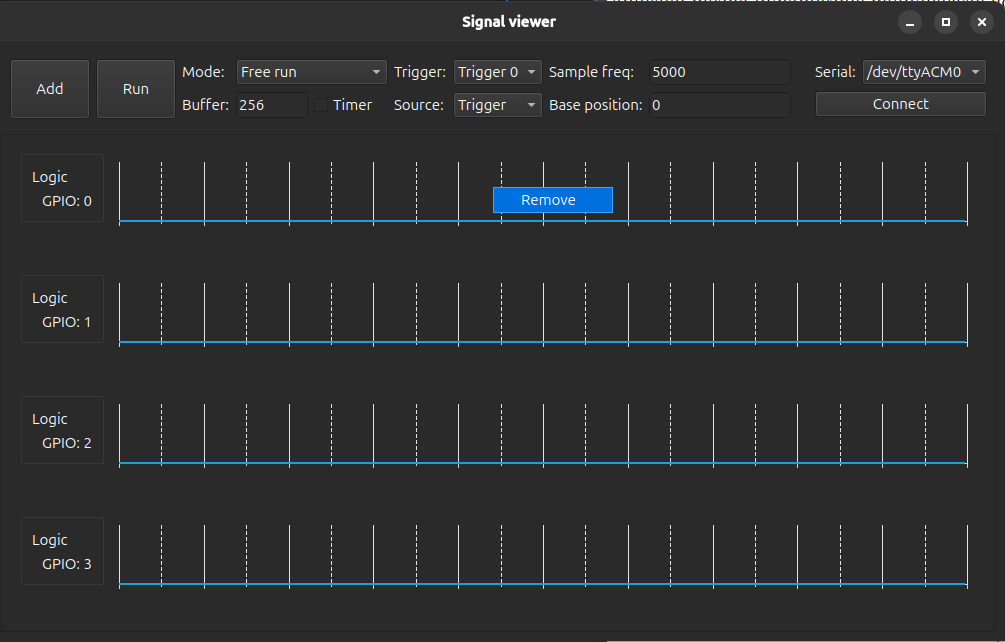
\includegraphics[width = 0.8\textwidth]{GUI_remove.png}
            \caption{Usuwanie pierwszego wykresu}
            \label{fig:gui_removePlot}
        \end{figure}

    
    \subsection{Pomiary}
        W celu rozpoczęcia pomiarów, należy podłączyć analizator do komputera, 
        następnie z listy rozsuwanej po prawej stonie wybrać port szeregowy,
        pod którym przedstawiło się urządzenie.

        W momencie podłączenia urządzenia do komputera zapala się zielona dioda na PCB informująca o zasilaniu układu a także
        druga zielona dioda LED tym razem dostępna na Raspberry Pi Pico, której miganie symbolizuje poprawny start analizatora oraz gotowość do rozpoczęcia pomiarów.
        Następnie po wybraniu trybu pracy i wciśnięciu przycisku \textit{RUN} w aplikacji graficznej, analizator rozpoczyna pracę,
        co sygnalizowane jest przez zatrzymanie się błyskającej diody.
    
    \subsection{Do dokończenia}
        Aktualna wersja aplikacji nie pozwala na komunikację sieciową, nie zawiera także implementacji Wyświetlanie sygnałów analogowych.

    \subsection{Błędy w kodzie}
        W aktualnej wersji GUI pozwala na analizowanie próbek cyfrowych, wybór trigger'a oraz dynamiczne generowanie wykresów.
        Jednak ze względu na błąd w kodzie, analizator nie zmienia częstotliwości próbkowania, podczas wybrania wewnętrznego wyzwalania - ustawiona jest domyślna częstotliwość 5kHz.
        
        Dodatkowo, podczas analizy wyzwalanej zewnętrznym trigger'em aplikacja czasami zamyka się z błędem \textit{,,IOT instruction (core dumped)''}.
        Problem ten, nie występuje podczas pracy na wewnętrznym taktowaniu.

        Ostatnim bugiem w aplikacji, jest niepoprawne czyszczenie bufora komunikacji przewodowej.
        Z jakiegoś powodu, czasem po próbie ponownego uruchomienia analizatora, ten nie reaguje na komendę startu.


